% This file was created by matlab2tikz.
%
%The latest updates can be retrieved from
%  http://www.mathworks.com/matlabcentral/fileexchange/22022-matlab2tikz-matlab2tikz
%where you can also make suggestions and rate matlab2tikz.
%
\definecolor{mycolor1}{rgb}{0.00000,0.44700,0.74100}%
\definecolor{mycolor2}{rgb}{0.85000,0.32500,0.09800}%
%
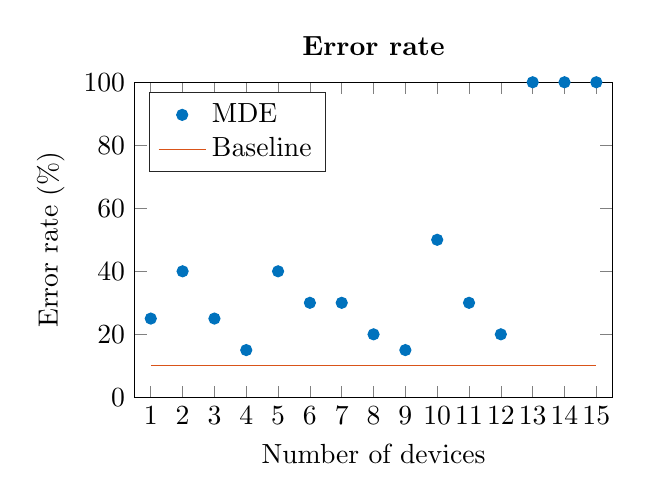
\begin{tikzpicture}

\begin{axis}[%
width=.5\textwidth,
height=.33\textwidth,
at={(0.758in,0.481in)},
scale only axis,
xmin=0.5,
xmax=15.5,
xtick={1,2,3,4,5,6,7,8,9,10,11,12,13,14,15},
xticklabels={{1},{2},{3},{4},{5},{6},{7},{8},{9},{10},{11},{12},{13},{14},{15}},
xlabel={Number of devices},
ymin=0,
ymax=100,
ylabel={Error rate (\%)},
axis background/.style={fill=white},
title style={font=\bfseries},
title={Error rate},
legend style={at={(0.03,0.97)},anchor=north west,legend cell align=left,align=left,draw=white!15!black}
]
\addplot [color=mycolor1,only marks,mark=*,mark options={solid}]
  table[row sep=crcr]{%
1	25\\
2	40\\
3	25\\
4	15\\
5	40\\
6	30\\
7	30\\
8	20\\
9	15\\
10	50\\
11	30\\
12	20\\
13	100\\
14	100\\
15	100\\
};
\addlegendentry{MDE};

\addplot [color=mycolor2,solid]
  table[row sep=crcr]{%
1	10\\
2	10\\
3	10\\
4	10\\
5	10\\
6	10\\
7	10\\
8	10\\
9	10\\
10	10\\
11	10\\
12	10\\
13	10\\
14	10\\
15	10\\
};
\addlegendentry{Baseline};

\end{axis}
\end{tikzpicture}%